\subsubsection{Phase 3: Erstellung von Object-Seiten}

Wie bereits im \autoref{subsec:entwurfsmuster} erwähnt, wird das Object
Page Entwurfsmuster für die Erstellung von Tests verwendet.
Vor der Implementierung des Szenarios muss der Tester zunächst
die Objekte und Seiten erstellen, die für die Ausführung des Szenarios
erforderlich sind. Im Rahmen des Registrierungstests müssen folgende
Seiten erstellt werden: LoginPage, RegistrationPage, ContractPage
(Privacy Policy) und die MainPage. Wenn die RegistrationPage
im Detail betrachtet wird, kann man feststellen, dass diese
Java-Klasse (wie alle anderen Object-Seiten) einige besondere Merkmale
aufweist.

Zunächst erbt sie von der Klasse Header (die den auf allen Seiten
vorhandenen Header repräsentiert). Der Header selbst stammt von
PageObject ab, das die Grundstruktur einer Seite repräsentiert
(siehe \Cref{fig:pag-uml}). Die Klassen Header und PageObject enthalten
Webelelemente und Methoden, die normalerweise auf allen Seiten der
Anwendung zugänglich sind. Dadurch kann das Design Pattern Page
Object optimal genutzt werden.

\begin{figure}[H]
    \centering
    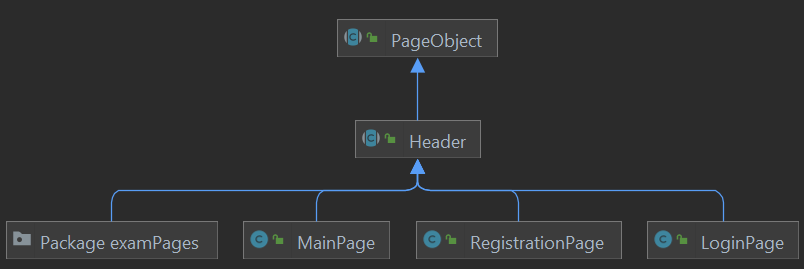
\includegraphics[scale=0.7]{images/pag-uml}
    \caption{UML Diagramm für die Java Page-Objekte} \label{fig:pag-uml}
\end{figure}

Zweitens enthält die Registrationpage eigene WebElemente.
Zum Beispiel die verschiedenen Inputs des auszufüllenden Formulars und
die anzuklickenden Bestätigungsbuttons (siehe Quellcode \ref{lst:registerpage}). Darüber hinaus
verfügt die Seite über die Methode registerUser, die ein
Formularobjekt (RegistrationForm) als Parameter hat und alle Eingaben
des Formulars ausfüllt und die ContractPage zurückgibt.

\begin{lstlisting}[label={lst:registerpage}, caption={RegistrationPage Quellcode}]
// RegistrationPage.java

    public class RegistrationPage extends Header {

    @FindBy(id = "cfirstname")
    private WebElement fieldFirstName;

    @FindBy(id = "csurname")
    private WebElement fieldName;

    @FindBy(id = "cmatrikel")
    private WebElement matrikel;

    public RegistrationPage(WebDriver driver) {
        super(driver);
    }

    @Override
    public boolean isInitialized() {
        WebElement h1_title;
        try{
            h1_title = driver.findElement(By.xpath("//H1[text()='Registrierung']"));
        }catch (NoSuchElementException e ){
            ExtentLogger.info("Main Title was not found");
            return false;
        }
        return h1_title.isDisplayed();
    }


    public ContractPage registerUser(RegistrationForm registrationForm){

        sendKeysToElement(fieldFirstName, registrationForm.firstName);
        sendKeysToElement(fieldName, registrationForm.lastName);

        Select fieldGender = new Select(driver.findElement(By.id("cgender")));
        fieldGender.selectByValue(registrationForm.gender);

        Select fieldCountry = new Select(driver.findElement(By.id("ccountry")));
        fieldCountry.selectByValue(registrationForm.country);

        Select fieldLanguage = new Select(driver.findElement(By.id("clanguage")));
        fieldLanguage.selectByValue(registrationForm.defaultLanguage);


        matrikel.clear();
        sendKeysToElement(matrikel, registrationForm.matrikel);

        Select fieldFaculty = new Select(driver.findElement(By.id("ou-combo")));
        fieldFaculty.selectByValue(registrationForm.faculty);

        Select fieldDegree = new Select(driver.findElement(By.id("degree-combo")));
        fieldDegree.selectByValue(registrationForm.degree);

        Select fieldExamReg = new Select(driver.findElement(By.id("er-combo")));
        fieldExamReg.selectByValue(registrationForm.examRegulation);

        WebElement addFaculty = driver.findElement(By.id("addEr"));

        clickElement(addFaculty);

        WebElement validationBtn = driver.findElement(By.xpath("(//INPUT[@class='btn fill-primary'])[2]"));
        clickElement(validationBtn);

        return new ContractPage(driver);
    }
}
\end{lstlisting}